\documentclass[11pt]{article}
\usepackage[utf8]{inputenc}
\usepackage{color}
\usepackage{amsmath}
\usepackage{algorithm}
\usepackage{algorithmic}
\usepackage{subfiles}
\usepackage{titling}
\usepackage{geometry}
\usepackage{graphicx}
\usepackage{xspace}
\usepackage{docmute}
\usepackage{lipsum}
\usepackage{makecell}
\usepackage{ragged2e}
\usepackage{multirow}
\usepackage{paralist}
\usepackage[dvipsnames]{xcolor}
\fboxsep0pt

\usepackage{caption}
\usepackage{glossaries}

\usepackage{hyperref}
\hypersetup{
  colorlinks=true,
  linkcolor=blue,
  filecolor=magenta,      
  urlcolor=cyan,
  pdftitle={This test},
  pdfpagemode=FullScreen,
}
\urlstyle{same}

\renewcommand{\labelenumii}{\arabic{enumi}.\arabic{enumii}}


\begin{document}
\begin{figure}
    \centering
    
\includegraphics[width=14cm]{Concordia-logo.jpeg}
    \label{fig:Concordia}
\end{figure}

\title{\textbf{SOEN 6841 \\ \vspace{\baselineskip}  TOPIC ANALYSIS AND SYNTHESIS (TAS)
\\\vspace{\baselineskip}We Are Project
\\Managers, Not
\\Superheroes}}
\author{Preet Angad Singh Nanda}
\date{November 2023}

\maketitle
\centering{\href{https://github.com/PreetAngadSingh/TAS-SOEN6841}{Github Link}}
\pagebreak
\tableofcontents

\pagebreak
\justifying
\section{Abstract}
In the dynamic realm of project management, this study explores the vital role of project managers, emphasizing their human qualities over superhero expectations. Focused on challenges in information technology environments, a three-step approach is proposed: recognizing personal strengths, understanding team dynamics, and forming strategic partnerships.

The study integrates insights from project management literature, Schock-Smith's analysis, and case studies, providing practical recommendations. Results show the approach thrives in dynamic environments, fostering improved team morale and efficient decision-making. Constraints include the need for open communication.

Future works aim at tools for self-assessment and team evaluation, addressing limitations in hierarchical structures and tight timelines. This study contributes nuanced insights for project managers, promoting a balanced perspective on achieving success in diverse project scenarios.

\section{Introduction}
In the dynamic landscape of project management, professionals often find themselves navigating complex challenges in various domains \cite{Williams2011}. This report delves into a critical aspect of project management highlighted by Angyne J. Schock-Smith in her contribution to the book "97 Things Every Project Manager Should Know" \cite{SchockSmith2017}. The focal point is the reminder that project managers are not superheroes but individuals with distinct strengths and weaknesses. Schock-Smith emphasizes the importance of self-awareness, team understanding, and skillful collaboration as keys to successful project management.

\subsection{Motivation}
The motivation behind investigating this concept stems from the recognition that project managers play a pivotal role in the success of any project, especially in the software and information technology environments \cite{Levitt2011}. The acknowledgment that project managers are not superheroes sets the stage for a deeper exploration into the traits and skills required for effective project management. Understanding one's limitations and strengths, as well as those of the team, is crucial for achieving project goals and ensuring a balanced, collaborative work environment.

In the fast-paced and ever-evolving field of project management, acknowledging the human aspect of the role becomes a motivational force \cite{Horine2009}. By recognizing that project managers are fallible individuals, the investigation seeks to uncover practical strategies to enhance project management effectiveness and foster a more resilient and adaptable approach to various challenges.

\subsection{Problem Statement}
The investigation addresses the challenge of unrealistic expectations placed on project managers, expecting them to be omnipotent and flawless in their decision-making \cite{Pollack2007}. This unrealistic perception can lead to burnout, stress, and ultimately hinder the success of projects. The problem at hand is the need to shift this perception and highlight the importance of acknowledging individual strengths and weaknesses in both the project manager and the team.

Precisely, the investigation aims to explore how project managers can navigate their roles more effectively by embracing their limitations and leveraging the diverse strengths within their teams. This involves understanding the problem of unrealistic expectations, identifying personal and team-related challenges, and proposing practical solutions for a more sustainable and successful project management approach.

\subsection{Objectives}
The primary objectives of this investigation are as follows:
\begin{itemize}
\item \textbf{Promote Self-awareness} Encourage project managers to reflect on their personal strengths and weaknesses through the exploration of past evaluations and assessments  \cite{SchockSmith2017}.
\item \textbf{Facilitate Team Understanding} Emphasize the significance of comprehending the strengths and weaknesses of team members to create a well-rounded and complementary project team \cite{ProjectManagementInstitute2009}.
\item \textbf{Enhance Collaboration} Provide insights into how project managers can use self-awareness and team understanding to foster collaborative partnerships that leverage individual strengths, thereby addressing weaknesses collectively \cite{Zulch2014}.
\item \textbf{Improve Project Outcome} Ultimately, the investigation aims to contribute to improved project outcomes by promoting a realistic and balanced approach to project management that recognizes and embraces the human element \cite{JohnsonLinkedIn}.
\end{itemize}
By achieving these objectives, the investigation aims to benefit project managers, team members, and organizations by fostering a healthier and more effective project management environment. The report seeks to provide actionable insights that contribute to the professional development of project managers and the overall success of diverse projects \cite{Simplilearn}.

\section{Background Material}
\subsection{The Role of Project Managers in Information Technology Environments}
Understanding the unique challenges faced by project managers in information technology environments is crucial. This subject explores the expectations, responsibilities, and common issues encountered by project managers in the IT sector. It includes an analysis of the evolving nature of technology projects and the increasing demand for effective project management in this dynamic field \cite{Williams2011}.

\subsection{The Importance of Self-awareness and Team Dynamics in Project Management}
This subject delves into the psychological aspects of project management, emphasizing the significance of self-awareness for project managers. It explores how an understanding of personal strengths and weaknesses, as well as those of team members, can contribute to successful project outcomes. The subject highlights the human side of project management and its impact on team collaboration and project success \cite{SchockSmith2017}.

\subsection{The Evolution of Project Management Methodologies in Information Technology}
This subject explores the historical development and evolution of project management methodologies within the realm of information technology. It delves into how traditional project management approaches have adapted to the unique challenges posed by IT projects, including rapid technological advancements, complex stakeholder landscapes, and evolving client expectations \cite{Pollack2007}. Understanding this evolution provides context for the challenges faced by modern project managers.

\subsection{Team Dynamics and Collaboration Strategies in Project Management}
This subject focuses on the intricacies of team dynamics within project management. It examines various models and theories related to team collaboration, communication, and conflict resolution. By understanding the psychological and interpersonal aspects of team interactions, project managers can foster a positive and productive working environment \cite{Zulch2014}. This subject complements the emphasis on self-awareness and team understanding, providing a deeper exploration of strategies for effective teamwork in project settings.

\section{Methods \& Methodology}
\subsection{The methodology of project management}
Project management is defined as the application of a body of knowledge, skills, tools, and techniques to project activities to meet project requirements \cite{ProjectManagementInstitute2009}. Effective project management necessitates an understanding of the project's environment (technology, industry, etc.) and general managerial abilities and interpersonal skills, in addition to the five project management procedures: initiating, planning, executing, monitoring and controlling, and closing \cite{Horine2009}. Today's successful project manager must possess these interpersonal skills, especially communication and leadership abilities, as a significant amount of project work frequently occurs in virtual environments.

\subsection{Approach to the Problem}
To address the problem at hand, a multifaceted approach was adopted. The investigation involved a comprehensive review of existing literature on project management, focusing on the challenges faced by project managers in various industries, with a specific emphasis on information technology. Additionally, an analysis of Schock-Smith's insights and strategies was conducted to derive practical methods for project managers to embrace their roles realistically \cite{SchockSmith2017}.

\subsection{Techniques Used in Analysis of Results}
The analysis involved qualitative methods, including the examination of Schock-Smith's three-part approach: self-awareness, team understanding, and collaborative partnerships. Case studies of successful project management experiences were also reviewed to identify patterns and effective strategies. The synthesis of these qualitative data points provided a basis for practical recommendations.


\section{Results Obtained}
The proposed three-part approach to project management is most effective in dynamic and adaptive project environments where change is frequent, and collaboration is paramount. It has shown significant success in information technology projects, where the ability to pivot and respond swiftly to emerging challenges is essential. This approach is particularly relevant when dealing with projects characterized by evolving requirements, diverse stakeholder involvement, and a need for continuous innovation \cite{SchockSmith2017}.

\subsection{Constraints}
While the approach offers substantial benefits, there are inherent constraints. Successful implementation relies heavily on open communication within the team. The necessity for team members to be transparent about their strengths and weaknesses, coupled with a willingness to engage in honest self-assessment, can be challenging in certain organizational cultures. Additionally, the effectiveness of the approach is contingent on the commitment of all team members to the collaborative process, and any lack of commitment may hinder its success \cite{Barrett2006}.

\subsubsection{Communication Skills and Leadership}
Barrett (2006b) claims that leadership communication is a multi-layered process that involves applying fundamental strategy development, effective writing and speaking abilities to more complicated organizational settings.
As a project progresses, the project manager must enhance their fundamental communication abilities to become more proficient in speaking.
Leadership communication can be explained as follows:
\begin{itemize}
\item \textbf{Core communication} The fundamental ability at the core of the spiral is the foundation for all successful communication. These are the more specialized abilities. Any organization's leaders need to be proficient in the fundamental abilities.
\item \textbf{Managerial Communication} The fundamental skills are reinforced by managerial communication qualities. It is the skills that are more directly related to overseeing others. It is the set of abilities required to lead teams and communicate with people.
\item \textbf{Corporate communication} Corporate communication involves expansion from the managerial skills to those abilities needed to lead an organization and address a broader community (Figure \ref{leadership communication}) \cite{Barrett2006}.
\end{itemize}

\begin{figure}[htbp]
    \centering
    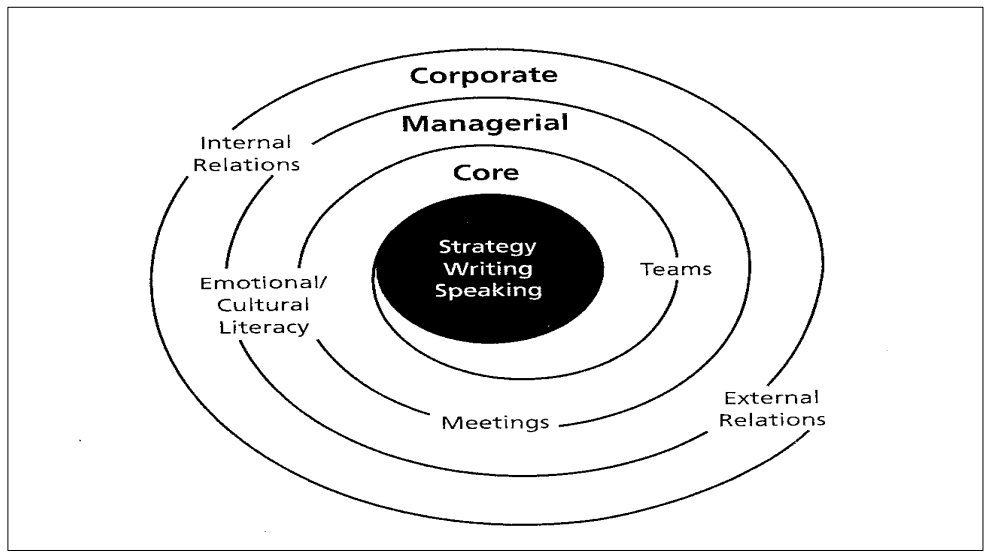
\includegraphics[width=8cm]{pic.png}
    \label{fig:Framework}
    \caption{\label{leadership communication}Leadership communication framework \cite{Barrett2006}}
\end{figure}

\subsection{Quality}
The quality of the results is considered adequate, and in some instances, exemplary, based on the combination of theoretical insights and practical strategies derived from real-world experiences. The approach provides a valuable framework for project managers, fostering an environment conducive to successful project outcomes. However, it is essential to recognize that the quality is contingent on the diligence and commitment of both the project manager and the team in implementing the proposed strategies.

\begin{figure}[htbp]
    \centering
    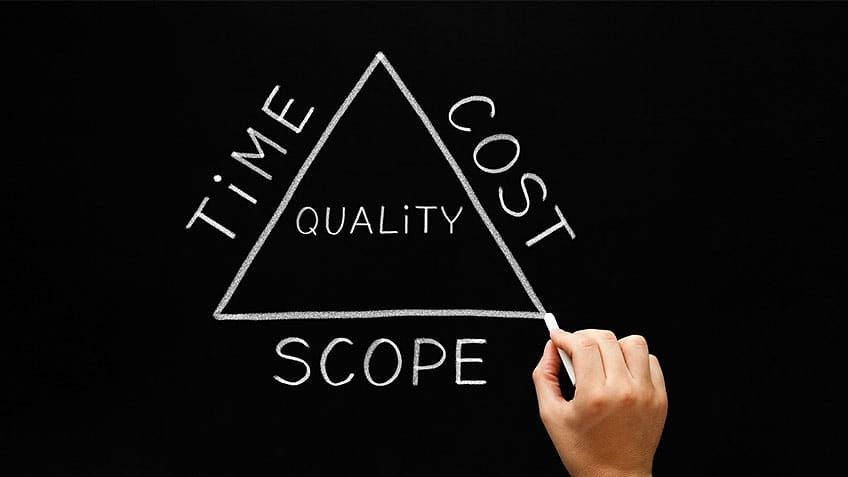
\includegraphics[width=11cm]{pic2.png.jpg}
    \label{fig:Framework}
    \caption{\label{three part approach}Three-part approach}
    \cite{Simplilearn}
\end{figure}

\subsection{Adaptability}
One notable strength of the results obtained is the adaptability of the proposed approach to various project contexts. While initially tailored to information technology environments, the principles can be seamlessly integrated into projects across diverse industries. This adaptability is a testament to the universality of the human aspects of project management, transcending specific sectors and methodologies.

\subsection{Long-Term Impact}
The results suggest that the adoption of this approach can have a lasting positive impact on project teams. Teams that embrace self-awareness, understand the dynamics of their members, and foster collaborative partnerships tend to exhibit higher morale, increased resilience in the face of challenges, and sustained productivity over the long term. The approach, when embedded in the organizational culture, has the potential to create a positive ripple effect, influencing not only individual projects but also contributing to an enhanced project management ecosystem within the organization.

\subsection{Continuous Improvement}
While the results are promising, there is room for continuous improvement. Future iterations of this approach could incorporate feedback mechanisms and ongoing assessments to ensure its relevance and effectiveness. This includes the development of tools and frameworks that facilitate real-time self-assessment and team evaluation, allowing project managers to adapt their strategies based on evolving project dynamics.

\subsection{Global Applicability}
The results obtained suggest that the proposed approach is not limited to specific geographic regions or cultural contexts. Its principles can be applied globally, making it a valuable asset for multinational organizations with diverse teams. The emphasis on understanding individual and team dynamics transcends cultural boundaries, contributing to a more inclusive and collaborative approach to project management on a global scale.

\section{Conclusions and Future Works}
\subsection{Suggested Improvements}
To augment the practicality of the proposed framework, future endeavors could delve into the development of user-friendly tools and training modules facilitating seamless self-assessment and team evaluation. Integrating emerging technologies, such as artificial intelligence, could offer objective insights, automating certain aspects of the process and making it more accessible to a broader range of project managers.

\subsection{Limitations to Solution}
While the outlined approach provides a valuable roadmap, its efficacy may be diminished in organizational cultures resistant to change or in highly bureaucratic structures that inhibit flexibility. Additionally, in time-sensitive projects, the thoroughness required for comprehensive self-assessment and team understanding may pose practical challenges. Recognizing these limitations ensures a nuanced application of the framework.

\subsection{Applications in Real World}
The proposed solutions find immediate application across diverse industries, especially in dynamic and innovation-driven sectors. IT projects, product development endeavors, and collaborative ventures stand to benefit significantly from adopting this approach. Beyond enhancing project outcomes, the framework fosters a positive team culture, improving overall organizational resilience and adaptability.

In the real world, the benefits extend beyond the immediate project scope. Improved team morale and communication efficiency contribute to a positive work environment, potentially reducing turnover rates and enhancing employee satisfaction. By acknowledging and embracing the inherently human aspects of project management, organizations can create resilient, high-performing teams capable of navigating the uncertainties inherent in contemporary project landscapes.

\subsection{Conclusion}
In essence, this investigation underscores the imperative for project managers to recognize their humanity and embrace their strengths and limitations. The three-part strategy proposed by Schock-Smith provides a practical guide for navigating the complexities of project management. By fostering self-awareness, understanding team dynamics, and strategically forming collaborative partnerships, project managers can transcend the myth of being superheroes and, instead, become adept leaders capable of steering projects towards success.
As we navigate the ever-evolving landscape of project management, this approach serves as a compass, guiding professionals through the intricacies of their roles. It is not a panacea but a robust foundation upon which adaptable and effective project management practices can be built. The insights gleaned from this investigation contribute to a holistic understanding of the multifaceted nature of project management, emphasizing the synergy between individual and collective strengths in achieving project success. Looking forward, continued exploration and refinement of these principles promise to enrich the field, fostering resilient project managers and high-performing teams in the face of evolving challenges.

\section{Critical Thinking and Research Approach}

Approaching the research topic, my focus was on unraveling the practical implications of project managers acknowledging their human limitations. Delving into Angyne J. Schock-Smith's three-part approach, I sought to understand its relevance beyond software project management and its potential for fostering effective collaboration in diverse projects.

Critical evaluation led me to question the seamless applicability of the approach in various organizational structures and fast-paced project scenarios. I considered the balance between open communication and the need for commitment within teams, recognizing potential challenges.

My research approach involved synthesizing Schock-Smith's insights with existing literature, analyzing case studies, and drawing connections to real-world challenges. This process aimed to provide a nuanced perspective on the human element in project management.

\section{Version Control System}
{\href{https://github.com/PreetAngadSingh/TAS-SOEN6841}{https://github.com/PreetAngadSingh/TAS-SOEN6841}}

\begin{thebibliography}{10}
    \bibitem{Levitt2011}Levitt, R. E. (2011). Towards project management 2.0. Engineering Project Organization Journal, 1(3), 197-210
    \bibitem{Pollack2007} Pollack, J. (2007). The changing paradigms of project management. International journal of project management, 25(3), 266-274.
    \bibitem{Zulch2014} Zulch, B. (2014). Leadership communication in project management. Procedia-Social and Behavioral Sciences, 119, 172-181.
    \bibitem{Barrett2006} Barrett, D.J. ( 2006b), Leadership communication: A communication approach for senior-level managers, In Handbook of Business Strategy, Emerald group publishing, Rice University, Houston
    \bibitem{Simplilearn} Simplilearn. (n.d.). Triple Constraints of Project Management. Retrieved from https://www.simplilearn.com/tutorials/project-management-tutorial/triple-constraints-of-project-management
    \bibitem{JohnsonLinkedIn} Johnson, D. The Missing Ingredient in Teamwork: How Self-awareness Leads to Success. Retrieved from https://www.linkedin.com/pulse/missing-ingredient-teamwork-how-self-awareness-leads-success-johnson/
    \bibitem{Williams2011} Williams van Rooij, S. (2011). Instructional design and project management: complementary or divergent?. Educational Technology Research and Development, 59, 139-158
    \bibitem{SchockSmith2017}We Are Project Managers, Not Superheroes 
    https://users.encs.concordia.ca/~kamthan/courses/soen-6841/topics/114.pdf
    \bibitem{ProjectManagementInstitute2009} Project Management Institute. (2009). A guide to the project management body of knowledge (PMBOK Guide) (4th ed.). Newton Square: Project Management Institute.
    \bibitem{Horine2009} Horine, G. (2009). Absolute beginner’s guide to project management (2nd ed.). Indianapolis: Que Publishing.
\end{thebibliography}
\end{document}
